% !TeX root = RJwrapper.tex
\title{\code{R} package \pkg{GofCens}: Goodness-of-Fit Methods for Right-Censored Data}
\author{by Mireia Besal\'u, Klaus Langohr, Matilde Fransciso, Arnau Garcia-Fernández, and Guadalupe G\'omez Melis}

\maketitle

\begin{abstract}
This paper presents the \code{R} package \pkg{GofCens}, which offers graphical tools and implements goodness-of-fit tests for  right-censored data. The first part provides a thorough  review of current methodologies for assessing goodness of fit in the presence of  right-censored data. The subsequent sections  present the main functions of \pkg{GofCens}  and are  illustrated by means of a right-censored sample from a log-normal distribution and a data set on NBA players' mortality, which is included in the package.
\end{abstract}

\section{Introduction}
Goodness-of-fit techniques are important to test the validity of parametric models and to ensure that the modeling assumptions hold true. Historically, goodness-of-fit tests have been developed for complete data, that is, when all the individual sample measurements have been observed. {The} Kolmogorov-Smirnov, Cram\'er-von Mises, and Anderson-Darling  statistics {are among the most commonly used goodness-of-fit tests. They} are based on a measure of the discrepancy between the empirical and  theoretical distribution functions. 

In order to account for censored data, these statistics  can be modified replacing the  empirical distribution function by the product-limit estimator of the distribution function. Modifications of Kolmogorov-Smirnov statistics for censored or truncated data go back to \citet{FOOH} and \citet{KB}. Pioneer extensions of Cram\'er-von Mises and Anderson-Darling  goodness-of-fit statistics to account for random right-censored data  are found in \citet{pettitt76} and \citet{koziol76}. Concerning chi-squared tests, \citet{mihalko80} propose an extension to censored data, specifically for type II right-censored data.

When the theoretical distribution function is completely specified and the data are uncensored, the above tests are all distribution-free, with known  distributions. However, this property no longer holds when data are censored or  when  the theoretical distribution function  involves unknown parameters. Moreover, there is no general  theory of asymptotic optimality in such cases \citep{lehmann05}. In fact, any test can achieve high asymptotic power or perform uniformly well  against local or contiguous alternatives, especially  when the family of possible alternatives is extensive \citep{janssen2000}. Given these limitations, graphical techniques have become a standard and straightforward way to assess distributional assumptions. They allow for a more intuitive examination of model fit. In addition, graphical methods complement formal goodness-of-fit tests. They often provide insights that the tests alone may not reveal.

The most well-known plots for assessing goodness-of-fit are probability plots. These include the Probability–Probability (P–P) plot, which compares the theoretical and estimated cumulative distribution functions, and the Quantile–Quantile (Q–Q) plot, which compares theoretical and estimated quantiles.
 There are also two alternatives to  these plots: the Stabilised Probability plot \citep{Mi}, which transforms the axes of the P-P plot to approximately get the same variance in each plotted point, and the Empirically Rescaled plot \citep{WT}, which is very useful when there is  a high percentage of random right-censored data.

{Goodness-of-fit methods for complete data and right-censored observations are widely available. However, many of these methods are not implemented in \code{R}, and those that are tend to be scattered across different packages.}
Among the publicly available computational tools in \code{R}, the \pkg{fitdistrplus} package \citep{DD, fitdistrplus1} provides the function \code{fitdistcens()}, which returns the result of the fit of any parametric distribution to a possibly right-censored data set. The function \code{cdfcomp()} of the same package can be used to graphically compare multiple fitted distributions with uncensored data.
{The} \code{probplot()} {function from} the \pkg{e1071} package \citep{e1071} generates probability plots for specified theoretical distribution. 
{Additionally, the} \code{distChooseCensored()} {function from the \pkg{EnvStats} package \citep{envstats, EnvStats1}} performs Shapiro-Wilk and Shapiro-Francia goodness-of-fit tests for normal, log-normal, and Gamma distributions, {handling both} complete and singly censored data \citep{Roy93}. 

In this work, we present the \code{R} package \pkg{GofCens} \citep{gofcens}, which provides various analytical methods and graphical tools to assess the goodness of fit of {parametric models} for non-negative,  right-censored lifetime data.  {These tools can also be applied to complete lifetime data.} Right censoring is restricted to type I or random censoring, and non-informative censoring is assumed for the failure time. In what follows, we review the analytical and graphical goodness-of-fit techniques for complete and right-censored data implemented in \pkg{GofCens}. Thereafter, the main functions of the \pkg{GofCens} package are presented and applied to a real data set, respectively. We conclude the paper with some final remarks on the current state of the package and possible enhancements.

\section{Methods}
\label{sec:methodse}

{Let $T$ denote the time to an event of interest, with distribution function $F$. The \pkg{GofCens} package provides goodness-of-fit methods to assess whether a univariate sample from $T$, either right-censored or complete, comes from a specified distribution family  $F_0(t; \theta)$, such as the Weibull, where $\theta$ is a vector of unknown parameters.}
Formally, the  null hypothesis in a  goodness-of-fit test is given by $H_0\!: F(t)=F_0(t;\theta)$. Specifically, the \pkg{GofCens} package provides implementations of  well-known tests such as  the Kolmogorov-Smirnov, Cram\'er-von Mises, and Anderson-Darling tests based on the empirical distribution function for complete data and their extensions for right-censored data. Additionally, \pkg{GofCens} includes a chi-squared-type test based on the squared differences between observed and expected counts using random cells, with  an extension tailored for right-censored data. Recognizing that these tests may not always yield high power, \pkg{GofCens} complements them with a series of graphical tools to aid in selecting the most suitable parametric model.

{Goodness-of-fit tests based on the empirical distribution function are typically developed under a fully specified null hypothesis $H_0\!: F(t) = F_0(t; \theta^*)$, such as a Weibull distribution with known parameters (e.g., $\alpha = 2$ and $\beta = 1$). They are less often formulated for the more general case $H_0\!: F(t)=F_0(t;\theta)$ , where $\theta$ is unknown. This distinction has important implications for how such tests are applied in practice.}
{This situation is common when fitting empirical data to parametric distributions with unknown parameters. To address it, we replace the unknown parameter $\theta$  with its maximum likelihood estimator $\hat\theta$. }
Following the recommendations in \citet{Cap09}, the implementation of the four tests ---Kolmogorov-Smirnov, Cram\'er-von Mises, Anderson-Darling, and chi-squared tests--- uses bootstrap techniques that involve the maximum-likelihood re-estimation of the unknown parameters $\theta$ in each simulated sample as we describe in Subsection Bootstrap methods.

In what follows, we briefly  outline the theory underlying these methods for testing $H_0\!: F(t) = F_0(t; \theta^*)$ assuming that the data consist of a sample of $n$ individuals,  each  subject to random right censoring. We denote by $T_1, \dotsc, T_n$ independent random variables with a common distribution  $F(\cdot)$ and by $C_1, \dotsc, C_n$ independent censoring  random variables with a common distribution $H(\cdot)$,  independent of $T_1, \dotsc, T_n$. The observed variables are defined  as  $Y_i = \min(T_i, C_i)$ and $\delta_i = \mathbf{1}\{T_i\leq C_i\},\, i = 1, \dotsc, n$.

\subsection{Tests based on empirical distribution functions}
\label{susec:tests}
In order to test $H_0\!: F(t) = F_0(t; \theta^*)$ for all $t\geq 0$, we can use statistics based on a distance between $F_0(t; \theta^*)$ and $\widehat{F}_n(t)$, the empirical distribution function for complete data, or either the Kaplan-Meier or the Nelson-Aalen estimator, if right-censored data are present. In both cases, large values of the distance indicate evidence against the hypothesized model.

\subsubsection{Kolmogorov-Smirnov test}
The Kolmogorov-Smirnov goodness-of-fit test is the most used analytical method to test goodness of fit when one is dealing with uncensored data. \citet{FOOH} published a modification of the Kolmogorov-Smirnov test in an attempt to obtain increased power when applied to uncensored data. They also generalized this test for  arbitrarily right-censored data.

For complete data, the Kolmogorov-Smirnov statistic is  defined as $D_n = \sup_t |\widehat{F}_n(t)- F_0(t; \theta^*)|$, where $\widehat{F}_n(t)$ is the empirical distribution function. To account for right-censored data, the Kolmogorov-Smirnov statistic is modified as
\begin{equation}
\label{eq:KSstat}
\widehat{D}_n = \sup_{0\leq t\leq t_m}  |\widehat{F}_n(t)-F_0(t; \theta^*)| =
  \sup_{0\leq t\leq t_m} \left|\int_0^t \frac{\widehat{S}_n(t)S_0(s; \theta^*)}{\widehat{S}_n(s)}d\big[\widehat{\Lambda}_n(s)-\Lambda_0(s; \theta^*)\big]\right|.
\end{equation}
{Here,} $\widehat{F}_n$, is replaced by $\widehat{F}_n = 1 - \widehat{S}_n = 1 - e^{-\widehat{\Lambda}_n}$, being $\widehat{\Lambda}_n$ the Nelson-Aalen estimator of the cumulative hazard function.  {In this case,} $S_0$ and $\Lambda_0$ {denote} the survival and the cumulative hazard function of the hypothesized distribution $F_0$, respectively, and $t_m$ is the largest observed time in the sample.

The standardized modified Kolmogorov-Smirnov statistic for censored data converges in distribution to $\sup_{0\leq t\leq F_0(t_m; \theta^*)} |B(F_0(t; \theta^*))|$, where $B(t)$ is a Brownian bridge. According to the results  in \citet{KB}, the asymptotic distribution of $\widehat{D}_n$ is given by
\begin{equation}
\label{eq:aprxKS}
  \lim_{n\rightarrow\infty} P(\sqrt{n}\widehat{D}_n\leq k) =
    \sum_{j = -\infty}^\infty (-1)^{j}e^{-2j^2k^2} P\Big(\Big|Z-2jk \sqrt{\frac{1-T}{T}} \Big| < k \sqrt{\frac{1}{T - T^2}}\Big),
\end{equation}
where $Z$ is a  standard normal random variable and $T = F_0(t_m; \theta^*)$.  An approximation for the $p$~value is proposed by \cite{FOOH}, which is considered acceptable when the $p$~value is less than 0.8 and excellent when it  is less than 0.2.

\subsubsection{Cram\'er-von Mises-type test}
\label{sususec:CvMtest}

{For uncensored data, }the Cram\'er-von Mises statistic is given by
\begin{equation*}
  M_n = n\int_{-\infty}^{+\infty}\big(\widehat{F}_n(t)-F_0(t; \theta^*)\big)^2dF_0(t).
\end{equation*}

For right-censored data, let $Y_1, \dotsc, Y_{n_r}$ represent  the $n_r$ observed failure times, that is, $\sum_{i = 1}^n \delta_i = n_r$. If we transform the order failure times $Y_{(1)}, \dotsc, Y_{(n_r)}$ into Uniform$(0,1)$ random variables $u_{(1)}, \dotsc, u_{(n_r)}$, defined as $u_{(i)} = F_0(Y_{(i)};\theta^*)$, and adopt the convention that $u_{(0)} = 0$ and $u_{(n_r + 1)} = 1$, we  can express the modified Cram\'er-von Mises statistic  as
\begin{equation}
\label{eq:CvMstat}
  \widehat{M}_n = n_r\sum_{j=1}^{n_r+1} \widehat{F}_n(u_{(j-1)})(u_{(j)}-u_{(j-1)}) \left(\widehat{F}_n(u_{(j-1)})-(u_{(j)}+u_{(j-1)})\right) + \frac{n_r}{3},
\end{equation}
which can be  easily computed. However, although the asymptotic distribution of $\widehat{M}_n$ has been studied by \citet{pettitt76} and \citet{koziol76}, its practical implementation is not straightforward.

\subsubsection{Anderson-Darling test}
\label{sususec:ADtest}
The Anderson-Darling test statistic is a modification of $M_n$ where the integrand is  weighted by the  inverse of $F_0(t)(1 - F_0(t))$:
\begin{equation*}
  A_n = n\int_{-\infty}^{+\infty}(\widehat{F}_n(t)-F_0(t; \theta^*))^2\frac{dF_0(t; \theta^*)}{F_0(t; \theta^*)(1-F_0(t; \theta^*)}.
\end{equation*}

For right-censored data, using the same notation as in the Cram\'er-von Mises statistic, the Anderson-Darling statistic is computed as
\begin{align}
\label{eq:ADstat}
\begin{split}
  \widehat{A}_n = -n_r &+ n_r\sum_{j = 1}^{n_r}(\widehat{F}_n(u_{(j - 1)}) - 1)^2 \left[\log|1 - u_{(j-1)}| - \log|1 - u_{(j)}|\right]\\
 &+ n_r\sum_{j=1}^{n_r-1}\widehat{F}_n^2(u_{(j)})\left[ \log |u_{(j+1)}| - \log |u_{(j)}| \right]-n_r\log|u_{(n)}|.
\end{split}
\end{align}
As with the Cramér-von Mises statistic, the asymptotic distribution of $\widehat{A}_n$ has been studied by \citet{pettitt76} but its practical implementation is not straightforward.

\subsubsection{Chi-squared type tests}
\label{susec:chisq}
\citet{Ki} introduced a general class of $\chi^2$ goodness-of-fit statistics for randomly right-censored data,   extending  Pearson's statistic where the cells are replaced by random cells.

Random cells are built as intervals in $\mathbb{R}$ whose  boundaries depend on some  sample summaries. These boundaries are defined by  a vector $\varphi$ of $r$ statistics, yielding intervals $I_j(\varphi)=(a_{j-1}(\varphi),\,a_{j}(\varphi)]$, where $j = 1, \dotsc, M$, and $-\infty=a_0(\varphi) < \, a_1(\varphi) \, < \,\dotsb < \, a_M(\varphi) = \infty$. For instance, we might take the quantiles $1/M,\, 2/M, \dotsc, 1$ as random cells boundaries $a_1(\varphi), \dotsc, a_M(\varphi)$.

The observed frequency of cell $j$, $N_{nj}(\varphi) = n\int_{I_j(\varphi)} d\widehat{F}_n$, is calculated using either the empirical distribution function or 1 minus the Kaplan-Meier estimator of the survival function if there are right-censored data. The expected probability of cell $j$ under the null hypothesis of a fully specified distribution, $F_0(t; \theta^*)$, is denoted by $p_j(\theta^*, \varphi_n)$.

The class of $\chi^2$ statistics is {defined} as
\begin{equation}
\label{eq:Chistat}
  T_n = V_n^\top(\theta^*, \varphi_n) \cdot K_n(\theta^*, \varphi_n)\cdot V_n(\theta^*,\varphi_n),
\end{equation}
where $K_n(\theta^*,\varphi)$ is a {symmetric, } non-negative definite matrix.{ $K_n(\theta^*,\varphi)$ is, in most cases, the inverse of a consistent estimator of the asymptotic variance-covariance matrix of the random vector $V_n(\theta^*,\varphi_n)$. The matrix can be computed following formulas (3.1) in \cite{Ki}}.  {The vector} $V_n(\theta^*,\varphi) = (\nu_{nj})_{j = 1, \dotsc, M}$, {contains  differences between observed and expected frequencies.
Each component is defined as} 
$$ \nu_{nj}(\theta^*, \varphi_n) = n^{-\frac12}N_{nj}(\varphi_n) - n^{\frac12} \cdot p_j(\theta^*, \varphi_n).$$ The limiting distribution of $T_n$ is a linear combination of independent noncentral $\chi^2$-distributed variables {which is complex to implement}. 

{\subsection{Computation of test statistic's distribution}}

{The limiting distributions of the statistics in  \eqref{eq:CvMstat}, \eqref{eq:ADstat}, and \eqref{eq:Chistat} under the null hypothesis $H_0\!: F(t) = F_0(t; \theta),$  when the parameter $\theta$ is unknown and replaced by its  maximum likelihood estimate  $\hat\theta$, are too complex to implement directly. Therefore, the corresponding  $p$~values are computed using bootstrap methods (see Subsubsection Bootstrap methods for right-censored data). For consistency, the $p$~values of the Kolmogorov-Smirnov test are also obtained using bootstrap.}

{The function \code{KScens()} of the \pkg{GofCens} package calculates the value of the test statistic of the Kolmogorov-Smirnov test, and, by default, approximates the $p$~value using bootstrap methods. Alternatively, the function also allows $p$~value computation based on the asymptotic distribution given in~\eqref{eq:aprxKS}.}
{The function \code{CvMcens()} in the \pkg{GofCens} package calculates the observed Cram\'er-von Mises statistic adapted for right-censored data, and provides an approximation of the corresponding  $p$~value using bootstrap methods.}
{The function \code{ADcens()} in the \pkg{GofCens} package  calculates the observed Anderson-Darling statistic for right-censored data and provides an approximation of the corresponding $p$~value using bootstrap methods.}
{The \code{chisqcens()} function in the \pkg{GofCens} package uses bootstrap techniques to compute the $p$~values.}

\subsubsection{Bootstrap methods for right-censored data}
\label{Subsec:Bootstrap}
Since the asymptotic distributions of the described goodness-of-fit statistics are unknown when the null hypothesis is not fully specified, bootstrap techniques offer a practical alternative for computing $p$~values. The bootstrap method is as well a practical alternative if $H_0$ is fully specified, but the asymptotic distribution depends on a complex expression. This section describes the application of bootstrapping to derive $p$~values for tests presented in the previous subsection. 
{
We use the notation $G_n$ to refer to any of the following test statistics: the Kolmogorov–Smirnov statistic defined in \eqref{eq:KSstat}, the Cramér–von Mises statistic in \eqref{eq:CvMstat}, the Anderson–Darling statistic in \eqref{eq:ADstat}, and the chi-squared statistic in \eqref{eq:Chistat}.
}

To test the null hypothesis $H_0\!:F(t) = F_0(t; \theta)$ using complete and right-censored data, we follow the guidelines of \citet{Cap09}. Accordingly, the observed data is utilized to estimate the parameter $\theta$, denoted as $\hat\theta_n$, using maximum likelihood estimation. Subsequently, we generate $B$ independent bootstrap samples of the same size ($n$) as the original data set as follows. Specifically, for each iteration $b$, $b = 1, \dotsc, B$, we compute the bootstrap statistic $(\widehat{G}_n^{\hat{\theta}_n})_b$  carrying out the following steps:
\begin{enumerate}
    \item Generation of survival times $T_1^b, \dotsc, T_n^b$ from the fitted distribution $F_0(t;\hat{\theta}_n)$.
    \item Generation of censoring times $C_1^b, \dotsc, C_n^b$ from the non-parametric estimation of $H$ obtained with the Kaplan-Meier estimator.
    \item Generation of observed survival times $Y_i^b = \min(T_i^b, C_i^b)$, and event indicators $\delta_i^b = \mathbf{1}\{T_i^b \le C_i^b\}, i = 1, \dotsc n$. 
    \item Maximum likelihood estimation of the parameter, $\hat{\theta}_n^b$, given $(Y_i^b, \delta_i^b), i = 1, \dotsc n$.  
    \item Computation of the bootstrap statistic, $(\widehat{G}_n^{\hat{\theta}_n})_b$.
\end{enumerate}

By repeating this process for many bootstrap samples ---the default value of the functions \code{KScens()}, \code{CvMcens()}, \code{ADcens()}, and \code{chisqcens()} is $B = 999$---, the sequence of bootstrap statistics, $(\widehat{G}_n^{\hat{\theta}_n})_b$, $b = 1, \cdots, B$, represents the empirical distribution of the statistic $G_n$ under the null hypothesis.

The $p$~value is calculated by comparing the observed test statistic $\widehat{G}_n$ to the empirical distribution of the bootstrap statistic. Specifically, the $p$~value is the proportion of bootstrap statistic values $(\widehat{G}_n^{\hat{\theta}_n})_b$ greater than or equal to the observed statistic $\widehat{G}_n$:
\begin{equation*}
  p = \frac{1}{B + 1} \big(\sum_{i=1}^B \mathbf{1}\{\widehat{G}_n \leq (\widehat{G}_n^{\hat{\theta}_n})_b\} + 1\big),
\end{equation*}
where adding 1 in both the numerator and the denominator avoids a zero $p$~value.

Note that steps 2 and 3, which involve generating the right-censored sample, are crucial. This is because the distribution of $G_n$ depends not only on $F_0$ but also on $H$ and the proportion of censored data. The functions \code{KScens()}, \code{CvMcens()}, \code{ADcens()}, and \code{chisqcens()} are designed so that, if the original data contains no right-censored observations, the censoring times in step 2 are automatically set to $\infty$. 

Moreover, as explained and illustrated in Section \lq Goodness-of-fit tests' below, these functions allow testing the null hypothesis of a fully specified choice of the parameters, $H_0\!:F(t) = F_0(t;\theta^*)$. In this case, the survival times in step 1 are generated from $F_0(t;\theta^*)$.

{\subsection{Goodness-of-fit plots}}

The \pkg{GofCens} package provides six different plots for evaluating goodness of fit, applicable to both right-censored and complete data. In most cases, a roughly straight line formed by the points suggests good agreement with the hypothesized theoretical distribution.

{\subsubsection{Probability-probability and Stabilized Probability plots}}

The probability-probability plot (P-P plot) maps $\widehat{F}_0(t)$ against $\widehat{F}_n(t)$, where $\widehat{F}_0(t)$ corresponds to either $F_0(t;\theta)$ with the unknown parameters replaced by their maximum likelihood estimates or to $F_0(t;\theta^*)$. $\widehat{F}_n$ represents either the empirical distribution function or 1 minus the Kaplan-Meier estimator of the survival function, if right-censored data are present.

In order to enhance the interpretability of the  P-P plot and because some of the plotted points have a larger variability than others, \citet{Mi} proposed the Stabilized Probability plot (SP plot). In the same way as the  $\arcsin$ transformation can be  used to stabilize the variance of a uniform order statistic, this function can be applied to stabilize the variance of $\widehat{F}_0(t)$. The variances of the resulting SP plotted points are all approximately equal.

{\subsubsection{Quantile-quantile plot}}
The quantile-quantile plot (Q-Q plot) maps the theoretical quantiles against the estimated quantiles, that is,  $\widehat{F}_0^{-1}(\widehat{F}_n(t))$ against $t$. An empirical rescaling of the axes can help to overcome the problem that the plotted points might not be evenly spread, in particular in the presence of right-censored data. The Empirically Rescaled plot (ER plot) plots $\widehat{F}_u(\widehat{F}_0^{-1}(\widehat{F}_n(t)))$ against $\widehat{F}_u(t)$, where $\widehat{F}_u(t)$ is the empirical cumulative distribution function of the points corresponding to the uncensored observations \citep{WT}.

Table \ref{tab:T1} provides an overview of the axes of the probability and quantile-quantile plots.
\begin{table}[!htpb]
\centering
\renewcommand{\arraystretch}{1.2}
\begin{tabular}{lcc}
 \toprule
  Plot & Abscissa & Ordinate\\
 \midrule
  P-P plot & $\widehat{F}_n(t)$ & $\widehat{F}_0(t)$ \\
  Q-Q plot & $t$ & $\widehat{F}_0^{-1}(\widehat{F}_n(t))$\\
  SP plot & $\frac{\pi}{2} \arcsin\big(\widehat{F}_n(t)^{\frac12}\big)$
          & $\frac{\pi}{2} \arcsin\big(\widehat{F}_0(t)^{\frac12}\big)$\\
  ER plot & $\widehat{F}_u(t)$ & $\widehat{F}_u(\widehat{F}_0^{-1}(\widehat{F}_n(t)))$ \\
 \bottomrule
\end{tabular}
\caption{Probability and quantile-quantile plots to assess goodness of fit.}
\label{tab:T1}
\end{table}

{\subsubsection{Cumulative  hazard  and Kaplan-Meier plots}}
Another set of plots consists of cumulative hazard plots, derived from transforming the cumulative hazard function $\Lambda$ in such a way that it becomes linear in $t$ or in $\log(t)$. The Nelson-Aalen estimator $\widehat{\Lambda}$ of $\Lambda$ is computed from the data, and the distribution-specific transformation $A(\widehat{\Lambda}(t))$ is then plotted against either $t$ or its natural logarithm. The transformations for all the distributions considered in the \pkg{GofCens} package are detailed in Table \ref{tab:dists}.

In addition, the \pkg{GofCens} package includes a function to graphically compare the Kaplan-Meier estimate of the survival function ($1 - \widehat{F}_n(t)$) with the parametric estimations of the survival function from the parametric models under study ($1 - \widehat{F}_0(t)$).  

\begin{table}[!h]
\centering
\setlength{\tabcolsep}{3pt}
\renewcommand{\arraystretch}{2.1}
\begin{tabular}{p{2cm}ccc}
 \toprule
  Distribution & Survival function  & Cum. hazard function & Plot \\[-4pt]
 \midrule
  Exponential [Exp$(\beta)$] & $\displaystyle e^{-\frac{t}{\beta}}$ & $\frac{t}{\beta}$
                             & $\widehat{\Lambda}(t)$ vs $t$\\
  Weibull [Wei($\alpha,\,\beta$)] & $\displaystyle e^{-(\frac{t}{\beta})^\alpha}$ & $(\frac{t}{\beta})^\alpha$
                                  & $\log \widehat{\Lambda}(t)$ vs $\log t$ \\
  Gumbel [Gum($\mu,\,\beta$)] & $\displaystyle 1 - e^{-e^{-\frac{t-\mu}{\beta}}}$
                              & $-\log\big(1 - e^{-e^{-\frac{t-\mu}{\beta}}}\big)$
                              & $-\log\big(\!-\log(1 - e^{-\widehat{\Lambda}(t)})\big)$ vs $t$ \\
  Log-Logistic [LLogis($\alpha, \beta$)] & $\displaystyle \frac{1}{1 + \left(\frac{t}{\beta}\right)^\alpha}$
                                         & $\log\big(1 + \big(\frac{t}{\beta}\big)^\alpha\big)$
                                         & $\log\big(e^{\widehat{\Lambda}(t)} - 1\big)$ vs $\log t$\\
  Logistic [Logis($\mu,\beta$)] & $\displaystyle \frac{e^{-\frac{t -\mu}{\beta}}}{1 + e^{-\frac{t - \mu}{\beta}}}$
                                & $\log\big(1 + e^{-\frac{t - \mu}{\beta}}\big)$
                                & $\log\big(e^{\widehat{\Lambda}(t)} - 1\big)$ vs $t$\\
  Log-Normal [LN($\mu,\beta$)] & $\displaystyle\int\limits_{\frac{\log t - \mu}{\beta}}^\infty \!\frac{1}{\sqrt{2 \pi}}
                                  e^{-\frac{x^2}{2}}dx$
                               & $-\log\big(1-\Phi\big(\frac{\log t-\mu}{\beta}\big)\big)$
                               & $\Phi^{-1}\big(1-e^{-\widehat{\Lambda}(t)}\big)$ vs $\log t$\\
  Normal [N($\mu,\beta$)] & $\displaystyle \int\limits_t^\infty \! \frac{1}{\beta\sqrt{2\pi}}
                             e^{-\frac{(x - \mu)^2}{2 \beta^2}} dx$
                          & $-\log\big(1-\Phi\big(\frac{t-\mu}{\beta}\big)\big)$
                          & $\Phi^{-1}\big(1 - e^{-\widehat{\Lambda}(t)}\big)$ vs $t$\\
\mbox{4-Parameter} Beta [Beta($\alpha, \gamma, a, b$)]
                                & $\displaystyle 1 - \frac{B_{(\alpha, \gamma, a, b)}(t)}{B(\alpha, \gamma)}$
                                & $-\log\big(1 - \frac{B_{(\alpha, \gamma, a, b)}(t)}{B(\alpha,\gamma)}\big)$
                                & $B^{-1}_{(\alpha, \gamma, a, b)} \big(B(\alpha, \gamma)
                                   \big(1 - e^{-\widehat{\Lambda}(t)}\big)\big)$ vs $t$\\
 \bottomrule
\end{tabular}
\caption{List of the distributions that are implemented in the \pkg{GofCens} package. The last column shows the specific transformations of time and the estimated cumulative hazard function of the cumulative hazard plots, which are implemented by the function \code{cumhazPlot()}. The shape parameters are denoted by $\alpha > 0$ and $\gamma > 0$, the location parameter by $\mu \in \R$, and the scale parameter by $\beta > 0$. The time $t$ will be always positive. $B(\alpha, \gamma)$ denotes the Beta function and  $B_{(\alpha,\gamma, a, b)}(t) = \int_0^{\frac{t - a}{b - a}} u^{\alpha - 1} (1-u)^{\gamma - 1}du$.}
\label{tab:dists}
\end{table}

\section[The GofCens package]{The \pkg{GofCens} package}
\subsection{Installation and dependencies}
The \pkg{GofCens} package can easily be installed from any CRAN repository by running the \code{R} command
\begin{example}
R> install.packages("GofCens")
\end{example}

As shown on the corresponding web page of the CRAN (\url{https://cran.r-project.org/web/packages/GofCens/index.html}), \pkg{GofCens} depends on the packages \pkg{survival} \citep{survival} and \pkg{actuar} \citep{actuar, actuar1}. The former is needed to estimate the survival and cumulative hazard functions, whereas the latter implements several distributions that are not available in standard \code{R} packages. Additionally, \pkg{GofCens} imports functions from the following packages: the {\code{fitdist()} and} \code{fitdistcens()} functions of the \pkg{fitdistrplus} package \citep{DD, fitdistrplus1} provide the estimation of the distributions' parameters; the packages \pkg{ggplot2} \citep{ggplot2, ggplot21}, \pkg{gridExtra} \citep{gridextra}, and the base package \pkg{grid} are needed for several features of the graphical tools; and the bootstrap methods to compute the $p$~values of the Kolmogorov-Smirnov, Cramér-von Mises, Anderson-Darling, and chi-squared type tests are implemented with the function \code{boot()} of the \pkg{boot} package \citep{boot}. {Moreover, the \code{is()} function from the base package \pkg{methods} is used internally to verify object classes during function execution.}

\subsection{Package overview}
The \pkg{GofCens} package provides both graphical tools and statistical test functions to assess goodness of fit for the distributions shown in Table~\ref{tab:dists}. 

The graphical functions, which facilitate visual evaluation of the model adequacy, include: 
\begin{itemize}
  \item Function \code{probPlot()} draws the probability and quantile-quantile plots of Table~\ref{tab:T1}.
  \item Function \code{cumhazPlot()} draws the cumulative hazard plots of Table~\ref{tab:dists}.
  \item Function \code{kmPlot()} draws the Kaplan-Meier estimates of the survival function and overlays parametric fits of the survival function. 
\end{itemize}

The statistical test functions, {which implement goodness-of-fit tests,} include:
\begin{itemize}

  \item Function \code{KScens()} implements the Kolmogorov-Smirnov test adapted to right-censored data.
  \item Function \code{CvMcens()} implements the Cram\'er-von Mises test adapted to right-censored data using bootstrap techniques.
  \item Function \code{ADcens()} implements the Anderson-Darling test adapted to right-censored data using bootstrap techniques.
  \item Function \code{gofcens()} computes the test statistics of the Kolmogorov-Smirnov, Cram\'er-von Mises, and Anderson-Darling tests adapted to right-censored data and returns the corresponding $p$~values.
  \item Function \code{chisqcens()} implements the chi-squared type test based on random cells and using bootstrap techniques.
\end{itemize}
These functions share several features: {although they are primarily designed for right-censored data, they can also be applied to complete datasets.} {They} provide parameter estimates for the distributions under study {and support two input formats:} users can either provide vectors with the observed survival times and the corresponding event indicator, {or use the common formula interface with a \code{Surv} object.} Earlier versions of the functions were implemented in \code{R} by \citet{Fe}, \citet{MiB}, and \citet{garcia17}.

{Specific features of the statistical test functions include the following:
On the one hand, these functions can be used to assess the goodness of fit for any distribution, provided that the corresponding \code{p}\emph{name}, \code{d}\emph{name}, and \code{r}\emph{name} functions are available. On the other hand, they return test-specific objects for which \code{print}, \code{summary}, and \code{print.summary} methods are implemented.}

In addition, the \pkg{GofCens} package comes with a data frame called \code{nba}, which contains the survival times of 3962 former players of the National Basketball Association (NBA) until 2019. These data were analyzed previously by \citet{Mart}.

{\subsubsection{A simulated example}}
Following, we will present the main features of the eight functions and illustrate their use with simulated survival times. For this purpose, we generate 300 survival times from a log-normal distribution with location parameter $\mu = 2$ and scale parameter $\beta = 1$, i.e., $T \sim LN(2,\,1)$, and 300 censoring times from an exponential distribution with scale parameter $\beta = 20$, i.e, $C \sim Exp(20)$:
\begin{example}
R> set.seed(123)
R> survt <- round(rlnorm(300, 2, 1), 2)
R> censt <- round(rexp(300, 1 / 20), 2)
\end{example}
The observed right-censored survival times, $Y = \min(T,\,C)$, and the corresponding event indicators, $\delta = \mathbf{1}\{T \le C\}$, are computed as follows:

\begin{example}
R> times <- pmin(survt, censt)
R> delta <- as.numeric(survt <= censt)
\end{example}
In total, 106 (35.3\%) survival times of the generated sample are right-censored:

\begin{example}
R> table(delta)
  0   1
106 194
\end{example}

\subsection[Graphical tools: Functions probPlot(), cumhazPlot(), and kmPlot()]{Graphical tools: Functions \code{probPlot()}, \code{cumhazPlot()}, and \code{kmPlot()}}
\subsubsection[Function probPlot()]{Function \code{probPlot()}}
\label{susec:probplot}
The \code{probPlot()} function allows users to assess graphically how well any of the distributions in Table~\ref{tab:dists} fit to a sample of right-censored survival or complete times. For this purpose, the function implements the four probability and quantile-quantile plots in Table~\ref{tab:T1}. By default, the function draws all four plots, but provides users with the option to choose only a subset of these. {If the user does not provide specific distribution parameters, the maximum likelihood estimates are used to draw the plots.} One graphical feature of the function is the option for users to choose between the base package \pkg{graphics}, which is the default, and the \pkg{ggplot2} package for drawing the plots. In the former case, \code{probPlot()} internally calls the \code{par()} function, enabling users to set graphical parameters within the function call.

For the illustration of the \code{probPlot()} function, we assess how well the log-normal distribution (left panel of Figure~\ref{fig:iluprobplot}) and the Weibull distribution (right panel of Figure~\ref{fig:iluprobplot}) fit to the sample data. The four plots in the left panel show fairly straight lines, thus confirming that the underlying distribution is the log-normal distribution, whereas the plots in the right panel clearly show that the Weibull distribution would not be an adequate distribution to model the data.

The \code{R} code used to draw the plots in the left and right panels of Figure~\ref{fig:iluprobplot} is the following:

\begin{example}
R> library("GofCens")
R> probPlot(times, delta, distr = "lognormal", cex.lab = 1.3)
R> probPlot(times, delta, distr = "weibull", ggp = TRUE)
\end{example}

\begin{figure}[!ht]
  \centering
  \includegraphics[width = 0.49\textwidth]{Figures/Fig1Left}
  \hfill
  \includegraphics[width = 0.49\textwidth]{Figures/Fig1Right}
  \caption{Probability plots applied to a right-censored sample from a log-normal distribution assuming log-normal (left panel) and Weibull distributions (right panel). Both figures are drawn with the \code{probPlot()} function.}
  \label{fig:iluprobplot}
\end{figure}

To illustrate additional functionalities of this function, we apply it again to the data set to assess the suitability of fitting a log-normal distribution with parameters $\mu = 2$ and $\beta = 1$. For this purpose, we employ the \code{params0} argument, whose default value is \code{NULL}, to specify the parameter values. Additionally, the main argument is a \code{Surv} object and we utilize the \code{m} argument to display the four probability plots in a single row, as shown in Figure~\ref{fig:iluprobplot2}. From these plots, it becomes evident that this log-normal distribution does not fit well to the data. Furthermore, {we set \code{prnt = TRUE} so that} the function provides both the parameter values used in the probability plots and the maximum likelihood estimates of the parameters, together with the values of the Akaike (AIC) and the Bayesian (BIC) information criteria. 

\begin{example}
R> probPlot(Surv(times, delta) ~ 1, distr = "lognormal", m = matrix(1:4, 
+    nrow = 1), params0 = list(location = 2, scale = 1.5), ggp = TRUE, prnt = TRUE)

Distribution: log-normal 

Parameters used in probability plots:
Location: 2 
   Scale: 1.5 

Parameter estimates:
Location (se): 1.988 (0.058)
   Scale (se): 0.883 (0.045)

   AIC: 1266.899 
   BIC: 1274.307    
\end{example}

\begin{figure}[!htpb]
  \centering
  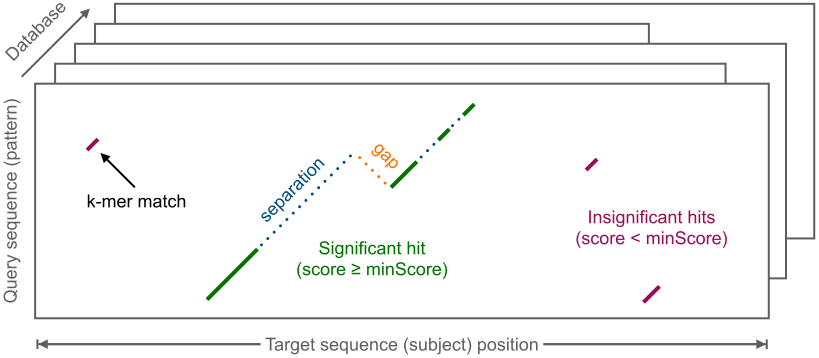
\includegraphics[width = 0.9\textwidth]{Figures/Fig2}
  \caption{Probability plots applied to a right-censored sample from a log-normal distribution assuming a log-normal distribution with specific parameters ($\mu = 2, \beta = 1.5$). The plots are drawn with the \code{probPlot()} function.}
  \label{fig:iluprobplot2}
\end{figure}

\subsubsection[Function cumhazPlot()]{Function \code{cumhazPlot()}}
\label{susec:cumhazplot}
The \code{cumhazPlot()} function can be used to generate cumulative hazard plots for any of the distributions listed in Table \ref{tab:dists}. As previously noted, the cumulative hazard plot is based on a transformation of the cumulative hazard function to achieve linearity in either $t$ or $\log(t)$. Consequently, given a set of survival times, this function serves as a useful tool to assess which parametric model best fits the data.

By default, the function generates cumulative hazard plots for the Weibull, Gumbel, log-logistic, logistic, log-normal, and normal distributions. Additionally, users can opt to choose the exponential and beta distributions or select any subset of these distributions. Similar to the \code{probPlot()} function, users can choose between the base \pkg{graphics} package (default) or \pkg{ggplot2} to draw the plots. 

{Setting the argument \code{prnt} to \code{TRUE} (default is \code{FALSE}),} the function also returns the maximum likelihood estimates for the specified distribution, along with the Akaike Information Criterion (AIC) and Bayesian Information Criterion (BIC) values.

An illustration with the previously generated right-censored sample from the log-normal distribution is shown in Figure~\ref{fig:ilucumhazplot}. As expected, the points of the cumulative hazard plot for the log-normal distribution show a fairly straight line, whereas most of the other distributions under study can clearly be discarded. This conclusion is further supported by comparing the AIC and BIC values across all distributions, with the log-normal distribution showing the lowest values.

The corresponding code is the following, where argument \code{degs = 2} is used to return the parameter estimates, which are shown below, with two decimal digits (default is \code{degs = 3}). 
\begin{example}
R> cumhazPlot(times, delta, font.lab = 4, cex.lab = 1.3, degs = 2, prnt = TRUE)

Parameter estimates

weibull
   Shape (se): 1.27 (0.07)
   Scale (se): 10.98 (0.62)
   AIC: 1304.05 
   BIC: 1311.45 

loglogistic
   Shape (se): 1.94 (0.11)
   Scale (se): 7.18 (0.42)
   AIC: 1272.48 
   BIC: 1279.89 

lognormal
Location (se): 1.99 (0.06)
   Scale (se): 0.88 (0.05)
   AIC: 1266.9 
   BIC: 1274.31 

gumbel
Location (se): 6.38 (0.33)
   Scale (se): 4.95 (0.3)
   AIC: 1342.49 
   BIC: 1349.9 

logistic
Location (se): 8.51 (0.43)
   Scale (se): 3.84 (0.23)
   AIC: 1430.25 
   BIC: 1437.66 

normal
Location (se): 9.89 (0.49)
   Scale (se): 7.54 (0.38)
   AIC: 1456.22 
   BIC: 1463.63 

\end{example}

\begin{figure}[!htpb]
  \centering
  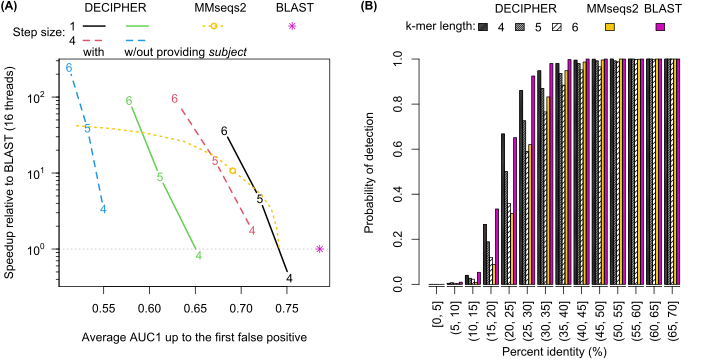
\includegraphics[width = 0.9\textwidth]{Figures/Fig3}
  \caption{Cumulative hazard plots for six different distribution applied to a right-censored sample from a log-normal distribution. The plots are drawn with the \code{cumhazPlot()} function.}
  \label{fig:ilucumhazplot}
\end{figure}

If users want to assess the goodness of fit of the exponential and the beta distribution and compare these with the fit of the log-normal distribution, they must specifically select these distributions, as shown in the following example. Notice that users need to provide the limits for the beta distribution, as the default domain, $(0,\,1)$, does not cover the range of the sample's survival times. In this example, plots are drawn using the \pkg{ggplot2} package (\code{ggp = TRUE}), and parameter estimates are not displayed on the screen.  The resulting plots are shown in Figure~\ref{fig:ilucumhazplot2}, where we observe that neither the exponential nor the beta distribution fits the data well. The corresponding \code{R} code is the following.

\begin{example}
R> cumhazPlot(times, delta, distr = c("exponential",  "beta", "lognormal"),
+    betaLimits = c(0, 100), ggp = TRUE)
\end{example}

\begin{figure}[!htpb]
  \centering
  \includegraphics[width = 0.9\textwidth]{Figures/Fig4}
  \caption{Cumulative hazard plots for the exponential, beta, and log-normal distribution applied to a right-censored sample from a log-normal distribution. The domain of the beta distribution is $(0,\,100)$.}
  \label{fig:ilucumhazplot2}
\end{figure}

\subsubsection[Function kmPlot()]{Function \code{kmPlot()}}
\label{susec:kmplot}
The \code{kmPlot()} function allows users to graphically compare the nonparametric Kaplan-Meier estimate of the survival function for a right-censored or complete sample of survival times with parametric estimates based on different models. For this purpose, each parametric estimate is individually overlaid on the Kaplan-Meier estimator of $S(t)$. Likewise the \code{cumhazPlot()} function, this is done by default for the Weibull, Gumbel, log-logistic, logistic, log-normal, and normal distributions, with the option to also include the exponential and beta distributions. The plots are generated using the \pkg{graphics} package by default, but setting \code{ggp = TRUE} enables the use of the \pkg{ggplot2} package. With both options, the pointwise 95\% confidence intervals are plotted. 

In the example shown in Figure~\ref{fig:kmplots}, the estimated survival functions for the six default distributions are overlaid on the nonparametric estimate of $S(t)$. As expected, the log-normal distribution exhibits the best fit to the data. However, based on these plots, the log-logistic distribution might also be considered as a parametric model that fits the sample data well.

The \code{R} code used to draw the Kaplan-Meier plots in Figure~\ref{fig:kmplots} is the following:

\begin{example}
R> kmPlot(times, delta, ggp = TRUE)
\end{example}

\begin{figure}[!ht]
  \centering
  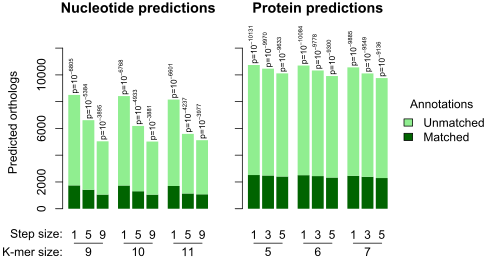
\includegraphics[width = 0.9\textwidth]{Figures/Fig5}
  \caption{Kaplan-Meier plots for six different distribution applied to a right-censored sample from a log-normal distribution. The shaded area represent the pointwise 95\% confidence intervals of the survival function. The plots are drawn with the \code{kmPlot()} function.}
  \label{fig:kmplots}
\end{figure}

{\subsection{Goodness-of-fit test functions}
\label{susec:goftests}}
In this section, we briefly describe and illustrate the use of the five functions in the \pkg{GofCens} package that implement the tests presented in the \lq Methods' section. 

{The basic \code{print} methods of} all functions {return the test statistic and the p-value, whereas the \code{summary} methods do also} provide the maximum likelihood estimates for the parameters of the hypothesized distribution $F_0(t; \theta)$ as well as the values of both the AIC and BIC. {The functions have also in common that} they offer the option to test the null hypothesis for specific parameter values of $F_0$, i.e., $F_0(t; \theta^*)$. {Each function returns an object of its own class, enabling the use of object-specific \code{print} and \code{summary} methods.}

\subsubsection[Function KScens()]{Function \code{KScens()}}
The \code{KScens()} function enables users to assess the goodness of fit using the Kolmogorov-Smirnov test adapted to right-censored data. It supports the eight distributions in Table~\ref{tab:dists} {as well as any other distribution for which the corresponding \code{p}\emph{name}, \code{d}\emph{name}, and \code{r}\emph{name} functions are implemented.} The function computes the test statistic in~(\ref{eq:KSstat}) and, by default, estimates the $p$~value using bootstrap methods. 

As illustrated below with the data from the generated right-censored sample, the function returns, by default, a list with {two} elements:
\begin{itemize}
  \item The null distribution.
  \item The test result, which includes the Kolmogorov-Smirnov test statistic (\code{A}) and the $p$~value.
\end{itemize}
{Additionally, the \code{summary} method provides two more elements:}
\begin{itemize}
  \item The maximum likelihood estimates of the parameters of the distribution under study.
  \item The values of the AIC and BIC.
\end{itemize}
In the illustration, we run the \code{KScens()} function to assess the goodness of fit of the log-normal and the Weibull distributions, first using bootstrapping to approximate the $p$~value, and second calculating the $p$~value following the results in \citet{FOOH}. Additionally, in the second example, we apply the function \code{summary} method, which {returns the parameter estimates, their standard errors and both the AIC and BIC.} As shown, the $p$~value obtained for the log-normal distribution is, as expected, larger (\code{0.115}) than the $p$~value (\code{0.042}) for the Weibull distribution. 
\begin{example}
R> set.seed(123)
R> KScens(times, delta, distr = "lognormal")

Null hypothesis: the data follows a lognormal distribution 

KS Test results:
      A p-value 
  0.781   0.115 
\end{example}

\begin{example}
R> set.seed(123)
R> summary(KScens(times, delta, distr = "weibull", boot = FALSE))

Distribution: weibull 

KS Test results:
      A p-value 
  1.391   0.042 

Parameter estimates (se):
shape             scale             
1.273 (0.067)     10.98 (0.621)     

AIC: 1304.046 
BIC: 1311.453
\end{example}

\subsubsection[Functions CvMcens() and ADcens()]{Functions \code{CvMcens()} and \code{ADcens()}}
The \code{CvMcens()} function calculates the test statistic of the Cram\'er-von Mises test in~(\ref{eq:CvMstat}), while the \code{ADcens()} function calculates the test statistic of the Anderson-Darling test in~(\ref{eq:ADstat}), and both employ bootstrap techniques to estimate the corresponding $p$~values. These functions share the same arguments, allowing users to specify the number of bootstrap samples, among other options. The default number of bootstrap samples for both functions is 999, which may result in lengthy computation times for large sample sizes. In such cases, users might consider reducing the number of bootstrap samples. For example, in the illustrations of the \code{CvMcens()} function below, with $n = 300$ and 999 bootstrap samples, the computation times are approximately 15 seconds using \code{R} version 4.5.0 on Windows 10 x64 (build 19045) with an Intel(R) Core(TM) i5-8500 processor (3.00 GHz).

The null hypotheses in the illustrations remain the same as before, as do the conclusions: we would conclude that the data may come from a log-normal distribution, but not from a Weibull distribution.

\begin{example}
R> set.seed(123)
R> summary(CvMcens(times, delta, distr = "lognormal"))

Distribution: lognormal 

CvM Test results:
    CvM p-value 
  0.054   0.450 

Parameter estimates (se):
location          scale             
1.988 (0.058)     0.883 (0.045)     

AIC: 1266.899 
BIC: 1274.307   
\end{example}

\begin{example}
R> set.seed(123)
R> summary(CvMcens(times, delta, distr = "weibull"))

Distribution: weibull 

CvM Test results:
    CvM p-value 
  0.376   0.001 

Parameter estimates (se):
shape             scale             
1.273 (0.067)     10.98 (0.621)     

AIC: 1304.046 
BIC: 1311.453  
\end{example}
Applying the function \code{ADcens()} in the same way as \code{CvMcens()}, the $p$~values are similar: $p = 0.52$ in the case of the log-normal distribution and $p = 0.001$ with the Weibull distribution.

Note that due to the use of resampling methods, with both functions it is advisable to previously set the seed of \code{R}'s random number generation in order to guarantee reproducibility of the test results. 

As mentioned before, users can also test the null hypothesis that the data come from a specific choice of the distribution under study, i.e., $H_0\!: F(t) = F_0(t; \theta^*)$. While this may be less relevant in practical applications, it can be useful for examining the properties of these tests. To perform such a test, users need to specify particular values for the distribution's parameters. For example, below we test the null hypothesis that the data follow a log-normal distribution with location and scale parameters $\mu = 2$ and $\beta = 1.5$. In this case, as shown, the Anderson-Darling test clearly rejects the null hypothesis (\code{p = 0.001}). Note that the output now includes both the specified parameter values for the null hypothesis and the maximum likelihood estimates. {In addition, we use the \code{outp} argument of the \code{summary.ADcens()} function to change the format of the output.}
\begin{example}
R> set.seed(123)
R> summary(ADcens(times, delta, distr = "lognormal",
+    params0 = list(location = 2, scale = 1.5)), outp = "table")

Distribution: lognormal 

Null hypothesis:
--------- | ---------
Parameter | Value    
--------- | ---------
location  | 2        
scale     | 1.5      
--------- | ---------

AD Test results:
------- | -------
Metric  | Value  
------- | -------
AD      | 9.536  
p-value | 0.001  
------- | -------

Parameter estimates:
--------- | --------- | ---------
Parameter | Value     | s.e.     
--------- | --------- | ---------
location  | 1.988     | 0.058    
scale     | 0.883     | 0.045    
--------- | --------- | ---------

AIC: 1266.899 
BIC: 1274.307 
\end{example}

\subsubsection[Function gofcens()]{Function \code{gofcens()}}
Rather than performing each of the three tests individually, users can run the Kolmogorov-Smirnov, Cramér-von Mises, and Anderson-Darling tests simultaneously with the \code{gofcens()} function, which calls each corresponding test function. This approach is especially useful for comparing the tests in a specific context or in a larger study, such as comparing their statistical power. However, a potential drawback is longer computation times, as each test function employs bootstrap methods to estimate the $p$~values. In the following examples, using the same data and null hypotheses as before, the computation time is approximately 20 seconds on \code{R} version 4.5.0, running on Windows 10 x64 (build 19045) with an Intel(R) Core(TM) i5-8500 processor (3.00 GHz). Note that in the second example, we modify options in the \code{summary.gofcens()} function: the number of bootstrap samples is displayed, while the AIC and BIC values are omitted.

\begin{example}
R> set.seed(123)
R> gofcens(times, delta, distr = "lognormal")

Null hypothesis: the data follows a lognormal distribution 

Test statistics
   KS   CvM    AD 
0.781 0.054 0.500 

p-values
   KS   CvM    AD 
0.115 0.450 0.520 
\end{example}
\begin{example}
R> set.seed(123)
R> summary(gofcens(times, delta, distr = "weibull"), print.AIC = FALSE,
+    print.BIC = FALSE, print.infoBoot = TRUE)

Distribution: weibull 

Test statistics
   KS   CvM    AD 
1.391 0.376 2.828 

p-values
   KS   CvM    AD 
0.001 0.001 0.001 

Parameter estimates (se):
shape             scale             
1.273 (0.067)     10.98 (0.621)     

Number of bootstrap samples: 999
\end{example}

\subsubsection[Function chisqcens()]{Function \code{chisqcens()}}
The \code{chisqcens()} function implements the chi-squared type test of \citet{Ki} explained in Section \lq Chi-squared type tests'. Likewise the \code{KScens()}, \code{CvMcens()}, and \code{ADcens()} functions, the computation of the $p$~value is achieved with bootstrap techniques using \code{BS = 999} as default value for the number of bootstrap samples. The function's {default} output includes the hypothesized distribution, the value of the test statistic, and the corresponding $p$~value. {The extended output provided by the \code{summary.chisqcens()} function also includes} the parameter estimates, the the AIC and BIC values {as well as} two values related to the number of random cells: the number initially chosen by the user (\code{Original}) and the final number used in the analysis (\code{Final}). The latter may be smaller due to the presence of right-censored data. For example, in the illustrations below using right-censored data from a log-normal distribution, we set \code{M = 8} random cells, but this number is reduced to \code{M = 7} due to censoring.

\begin{example}
R> set.seed(123)
R> chisqcens(times, delta, M = 8, distr = "lognormal")

Null hypothesis: the data follows a lognormal distribution 

Chi-squared Test results:
Statistic   p-value 
    3.123     0.154 

\end{example}
\begin{example}
R> set.seed(123)
R> summary(chisqcens(times, delta, M = 8, distr = "weibull"))

Distribution: weibull 

Chi-squared Test results:
Statistic   p-value 
    8.599     0.002 

Parameter estimates (se):
shape             scale             
1.273 (0.067)     10.98 (0.621)     

Cell numbers:
Original    Final 
       8        7 

AIC: 1304.046 
BIC: 1311.453 
\end{example}

Again, based on the outputs, we would choose the log-normal distribution instead of the Weibull distribution, because its value of the test statistic is clearly smaller (3.123 vs 8.599) and the $p$~value is far larger ($p = 0.154$ vs $p = 0.002$).

{The following illustration highlights two features of the goodness-of-fit test functions in the \pkg{GofCens} package. First, all functions return structured objects that can be stored as standard objects for further use in \code{R}. Second, users can test the goodness-of-fit of distributions different from the eight distributions in Table~\ref{tab:dists}. In this example, we apply the \code{chisqcens()} function using the gamma distribution. As shown, the parameter estimates are reported with the default names \code{theta1} and \code{theta2}, and the result is an object of class \code{chisqcens}, further processed with the \code{summary} method to display detailed results.}

\begin{example}
R> set.seed(123)
R> result <- summary(chisqcens(times, delta, M = 8, distr = "gamma")) 
R> result

Distribution: gamma 

Chi-squared Test results:
Statistic   p-value 
    6.176     0.006 

Parameter estimates (se):
theta1            theta2            
1.65 (0.144)     0.165 (0.019)     

Cell numbers:
Original    Final 
       8        7 

AIC: 1293.124 
BIC: 1300.532    
\end{example}
\begin{example}
R> class(result)

[1] "summary.chisqcens" "chisqcens"
\end{example}

\section{Real data example: Survival times of retired NBA players}
\label{sec:examples}
In this section, we apply several functions of the \pkg{GofCens} package to determine the parametric model that best fits the survival times of former NBA players.

The data frame \code{nba} comes with the {GofCens} package and contains the survival times (variable \code{survtime}) of all 3962 former players of the National Basketball Association (NBA) from its inception until July 2019. These data have been published and analyzed by \citet{Mart}, where survival times are measured as the elapsed time (in years) from the end of the NBA career until either death (\code{cens == 1}) or July 31, 2019 (\code{cens == 1}). By this date, 864 (21.8\%) of the former players had died, with uncensored post-NBA survival times ranging from a few days until nearly 70 years. The estimated median survival time is 54.1 years as shown below in the output of the function \code{npsurv} of the \pkg{rms} package \citep{rms} and Figure~\ref{fig:KMNBA}, which shows the Kaplan-Meier estimate of the survival function. 

\begin{example}
R> data("nba")
R> library("rms")
R> npsurv(Surv(survtime, cens) ~ 1, nba)

Call: npsurv(formula = Surv(survtime, cens) ~ 1, data = nba)
        n events median 0.95LCL 0.95UCL
[1,] 3962    864   54.1    53.1    55.1    
\end{example}

The \code{R} code to draw the plot in Figure~\ref{fig:KMNBA} is the following:
\begin{example}
R> par(las = 1, cex.lab = 1.3, cex.axis = 1.2, font.lab = 4, font.axis = 2,
+    mar = c(5, 5, 2, 2), yaxs = "i", xaxs = "i")
R> survplot(npsurv(Surv(survtime, cens) ~ 1, nba), lwd = 3,
+    xlab = "Years after NBA career", time.inc = 5, col.fill = grey(0.6),
+    ylab = "Estimated survival probability", xlim = c(0, 75))
R> abline(h = 0.5, lwd = 2, lty = 2)
\end{example}

\begin{figure}[!ht]
  \centering
  \includegraphics[width = 0.65\textwidth]{Figures/Fig6}
  \caption{Survival function of times from the end of the NBA career until death among retired  players. The shaded area represents the confidence bands of the survival function.}
  \label{fig:KMNBA}
\end{figure}

In order to model parametrically the survival times and estimate the median, we need to know
which distribution is the most appropriate distribution. For this purpose, we take advantage of the \code{cumhazPlot()} function, which provides the six cumulative hazard plots shown in Figure~\ref{fig:NBAcumhaz}:

\begin{example}
R> cumhazPlot(Surv(survtime, cens) ~ 1, nba, font.lab = 4, cex.lab = 1.3, 
+    lwd = 3, colour = "blue")
\end{example}

\begin{figure}[!ht]
  \centering
  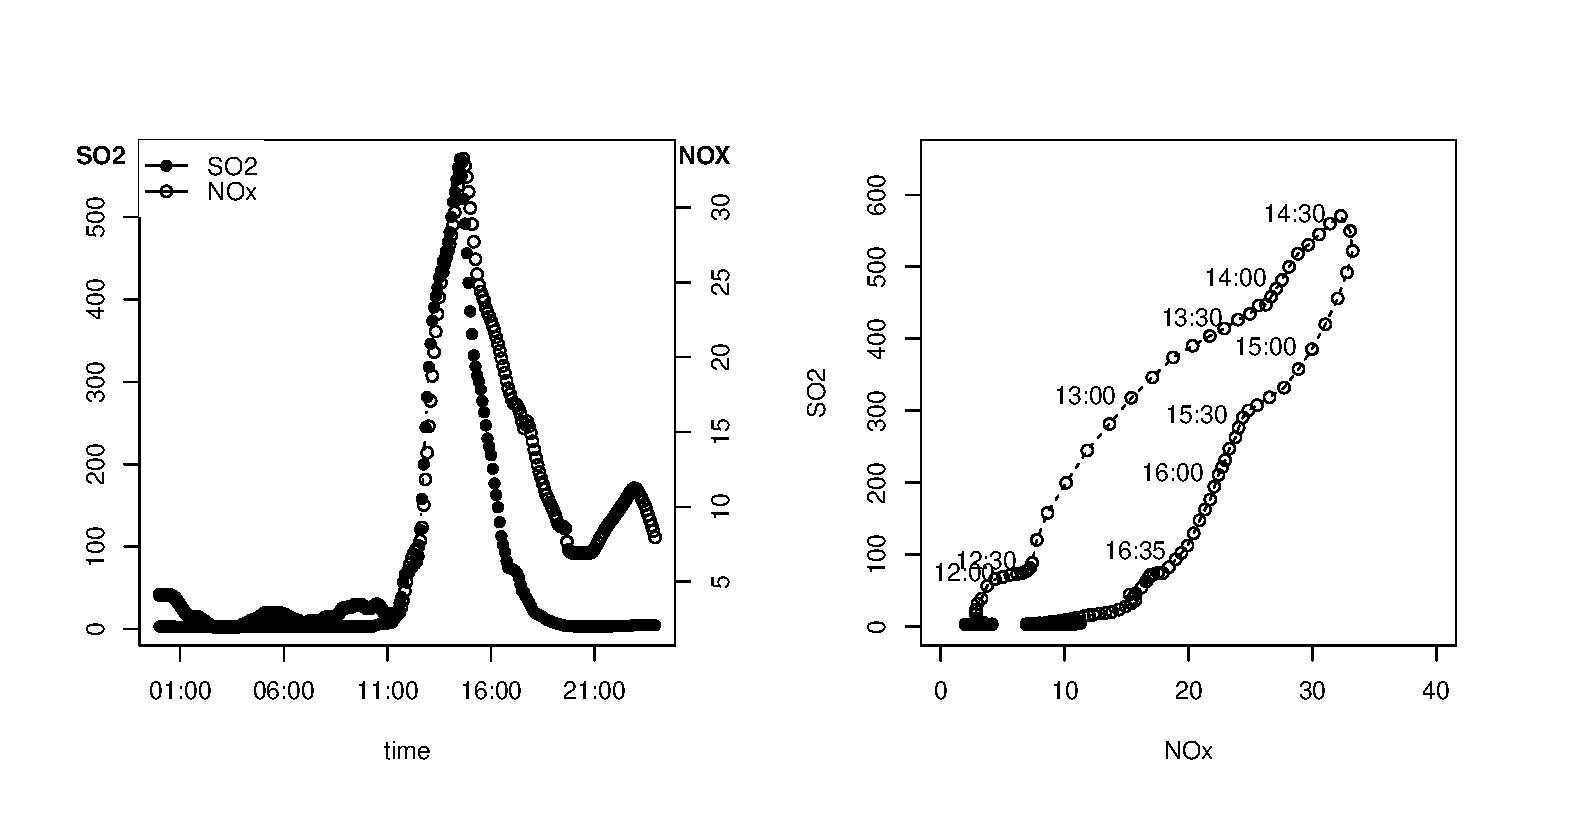
\includegraphics[width = 0.9\textwidth]{Figures/Fig7}
  \caption{Cumulative hazard plots for six different distributions applied to the survival times of former NBA players. The plots are generated with the \code{cumhazPlot()} function.}
  \label{fig:NBAcumhaz}
\end{figure}

According to the plots in Figure~\ref{fig:NBAcumhaz}, the logistic distribution fits reasonably well to the data, even though the corresponding plot does not show a completely straight line of the points. In addition, we could also consider the normal distribution for parametric analyses of the survival times. To choose one of either distributions, we run the following code to draw the probability and quantile-quantile plots that are shown in the left and right panels of Figure~\ref{fig:probplotNBA} with the \code{probPlot()} function. 
\begin{example}
R> probPlot(Surv(survtime, cens) ~ 1, nba, distr = "logistic", ggp = TRUE)
R> probPlot(Surv(survtime, cens) ~ 1, nba, distr = "normal", ggp = TRUE)
\end{example}

According to the plots in Figure~\ref{fig:probplotNBA}, the logistic distribution appears to be a slightly better choice than the normal distribution, as the points in all four plots on the right panel show some curvature. 

Note that in the previous function calls, we used the \code{formula} versions of both functions, which allows for the inclusion of the data frame \code{nba} in the argument list, which simplifies their use.

\begin{figure}[!ht]
  \centering
  \includegraphics[width = 0.48\textwidth]{Figures/Fig8left}
  \hfill
  \includegraphics[width = 0.48\textwidth]{Figures/Fig8right}
  \caption{Logistic and normal probability plots for the survival times of former NBA players. The plots are drawn with the \code{probPlot()} function.}
  \label{fig:probplotNBA}
\end{figure}

Finally, we apply the \code{gofcens()} function to both distributions in order to complement the plots with the results of the Kolmogorov-Smirnov, Cram\'er-von Mises, and Anderson-Darling tests. 

\begin{example}
R> set.seed(123)
R> summary(gofcens(Surv(survtime, cens) ~ 1, nba, distr = "logistic"))

Distribution: logistic 

Test statistics
    KS    CvM     AD 
 2.099  1.277 13.849 

p-values
   KS   CvM    AD 
0.001 0.009 0.002 

Parameter estimates (se):
location          scale             
53.077 (0.457)     9.013 (0.218)     

AIC: 8460.297 
BIC: 8472.866  
\end{example}

\begin{example}
R> set.seed(123)
R> summary(gofcens(Surv(survtime, cens) ~ 1, nba, distr = "normal"))

Distribution: normal 

Test statistics
    KS    CvM     AD 
 2.736  2.666 22.957 

p-values
   KS   CvM    AD 
0.001 0.002 0.001 

Parameter estimates (se):
location          scale             
53.004 (0.518)     16.977 (0.368)     

AIC: 8512.579 
BIC: 8525.148
\end{example}

Following the test results, we would reject the null hypothesis in both cases: the Kolmogorov-Smirnov, Cramér-von Mises, and Anderson-Darling tests all yield small $p$-values, indicating that neither the logistic nor the normal distribution are adequate models for the survival times of former NBA players. This result is not unexpected given the large sample size, which increases the power of the tests and makes even minor deviations from the model detectable. Despite the rejection, the diagnostic plots in Figures~\ref{fig:NBAcumhaz} and \ref{fig:probplotNBA} suggest that the logistic distribution provides a somewhat better fit to the data than the normal distribution. Therefore, it seems reasonable to use the logistic model as a practical approximation. Based on the maximum likelihood estimates, the fitted parameters are $\hat\mu = 53.08$ and $\hat\beta = 9.01$, yielding an estimated median survival time of approximately 53.1 years, which is close to the non-parametric estimate of 54.1 years.

\section{Conclusion}

In this paper we have presented the \code{R} package \pkg{GofCens}, whose functions offer both analytical methods and graphical tools to assess the goodness of fit for right-censored lifetime data. {While the graphical functions can be used to assess the goodness of fit for the eight distributions listed in Table~\ref{tab:dists}, which represent the most common ones in survival analysis, the goodness-of-fit test functions are more flexible and can be applied to any distribution available in \code{R}.} \pkg{GofCens} incorporates new functions for goodness-of-fit analyses while unifying functions that are otherwise scattered across various \code{R} packages. As shown with several examples, this package is a user-friendly tool that enables {users} to determine the most suitable parametric distribution for analyzing their data.

For the analysis of a given data set in practice, it is important to highlight the usefulness of including probability or cumulative hazards plots alongside the goodness-of-fit tests provided in \pkg{GofCens}. While statistical tests offer summary statistics, such plots offer a comprehensive view of the data, thus revealing peculiarities that might escape detection through summary statistics alone. Moreover, the importance of selecting a specific distribution depends on the context of the analysis. For example, precise distributional assumptions may be less critical when evaluating test statistics, but become essential when estimating quantiles or making extrapolations. The selection of any of the four tests presented herein is, to some extent, subjective, influenced by personal preference and convenience, as none of them emerges as optimal for all censoring situations, parametric families, or sample sizes.

{In recent years, additional goodness-of-fit techniques for right-censored data have been developed, including transformation-based procedures \citep{goldmann} and modifications of classical tests using pseudo-complete samples or randomization strategies \citep{balakrishnan2015}. While these methods can offer improved performance in specific settings, they often involve specialized implementation or focus on narrower applications. In contrast, \pkg{GofCens} implements established, flexible approaches with broad applicability and interpretability, supporting classical tests enhanced by resampling and graphical diagnostics.}

Feasible extensions of this package {include expanding the range of distributions supported by the graphical functions. Since, for example, the \code{cumhazPlot()} function requires distribution-specific transformations of the cumulative hazard function, such an extension is not straightforward.} {Additional developments} could involve adapting its functions to handle left-truncated and interval-censored data. Furthermore, exploring residual-based methods to assess the parametric assumptions an accelerated failure time model may be a promising direction for further development.

\section*{Acknowledgements}

M. Besalú's, G. Gómez Melis' and K. Langohr's research was funded by MICIU/AEI/10.13039/2501100011033 and FEDER, UE [PID2023-148033OB-C21] and  by  Agència de Gestió d'Ajuts Universitaris i de Recerca [2021 SGR 01421] (GRBIO) from Generalitat de Catalunya (Spain).

We thank the anonymous referees for their valuable and significant feedback.

\bibliography{RJreferences}

\address{Mireia Besal\'u\\
 {Department of Statistics and Operations Research, Biostatistics and Bioinformatics Group and Institute for Research and Innovation in Health (IRIS)}\\ Universitat Polit\`ecnica de Catalunya{· BarcelonaTech (UPC)} \\
  Jordi Girona 1-3, 08034 Barcelona\\
  Spain\\
  \url{https://orcid.org/0000-0003-0473-2404}\\
  \email{mireia.besalu@upc.edu}}

\address{Klaus Langohr\\
 {Department of Statistics and Operations Research, Biostatistics and Bioinformatics Group and Institute for Research and Innovation in Health (IRIS)}\\
  Universitat Polit\`ecnica de Catalunya{· BarcelonaTech (UPC)}\\
  Jordi Girona 1-3, 08034 Barcelona\\
  Spain\\
  \url{https://orcid.org/0000-0001-7075-9192}\\
  \email{klaus.langohr@upc.edu}}

\address{Matilde Francisco\\
 {Department of Statistics and Operations Research and Biostatistics and Bioinformatics Group,} \\
  Universitat Polit\`ecnica de Catalunya{· BarcelonaTech (UPC)}\\
  Jordi Girona 1-3, 08034 Barcelona\\
  Spain\\
  \url{https://orcid.org/0009-0009-1982-0547}\\
  \email{matilde.martins.da.palma@upc.edu}}

\address{Arnau Garcia-Fernández\\
 {Department of Statistics and Operations Research  and Biostatistics and Bioinformatics  Group
 }\\
  Universitat Polit\`ecnica de Catalunya{· BarcelonaTech (UPC)} \\
  Jordi Girona 1-3, 08034 Barcelona\\
  Spain\\
  \url{https://orcid.org/0009-0009-7370-6980}\\
  \email{arnau.garcia.fernandez@upc.edu}}

\address{Guadalupe G\'omez Melis\\
 {Department of Statistics and Operations Research, Biostatistics and Bioinformatics  Group and Institute for Research and Innovation in Health (IRIS)}\\
 Universitat Polit\`ecnica de Catalunya{· BarcelonaTech (UPC)} \\
  Jordi Girona 1-3, 08034 Barcelona\\
  Spain\\
  \url{https://orcid.org/0000-0003-4252-4884} \\
  \email{lupe.gomez@upc.edu}}
